\documentclass[UTF8,fontset=fandol,zihao=-4]{ctexart}
\usepackage[a4paper,margin=25mm]{geometry}
\usepackage{amsmath,amssymb,booktabs,array,graphicx,hyperref,xcolor}
\usepackage{caption,fancyhdr}
\hypersetup{colorlinks=true,linkcolor=blue,citecolor=blue,urlcolor=blue}
\setlength{\headheight}{15pt}
\setlength{\emergencystretch}{2em}
\pagestyle{fancy}\fancyhf{}\fancyhead[L]{ParallelBayes：软件与计算实验稿}\fancyfoot[C]{\thepage}
\newcommand{\E}{\mathbb{E}}
\newcommand{\R}{\mathbb{R}}
\title{ParallelBayes：时间并行 MCMC 的可核验实现与单机 CPU 基准}
\author{中文研究稿：作者与单位待定}
\date{2026 年 10 月}
\begin{document}
\maketitle
\begin{abstract}
时间并行马尔可夫链蒙特卡洛（MCMC）将轨迹递推改写为并行求解问题，但执行加速与可靠推断成本仍须分别评价。本文实现研究软件ParallelBayes，提供Stan与BridgeStan的CPU顺序RWM/MALA入口，并通过R控制接口对明确实现的原生JAX目标组织顺序核、窗口quasi-DEER、Online Picard和BlackJAX NUTS，并保存实际随机输入、数值核验及完整任务记录。在M4 Mac CPU上，冻结的八个目标、两个预算和每组24次独立重复共1920项任务全部完成，最大独立核验路径差为$2.36\times10^{-8}$，接受事件无失配。quasi-DEER与Picard的组中位完整工作流速度比分别为0.072--0.739和0.226--0.814，均未显示组中位加速。较长预算下，NUTS在五个目标上满足预声明函数误差阈值的逐点区间判据，两个MH核各为两个；中心化漏斗、多峰探索和有限参考仍限制结论。另完成64个新生成数据集的320次拟合；审查后解析对照显示，该批数据的解析90\%区间覆盖本身为54/64，并通过配对端点及现代链诊断定位有限采样偏差。小型CPU机制实验与独立环境复现另行登记。贡献是可重放的软件、计算核验和指定CPU条件下的跨模型证据；不声称新采样算法、通用加速或一般正确性证明。
\end{abstract}

\section{问题与研究范围}
时间并行 MCMC 的吸引力在于缩短单条指定轨迹的计算延迟。轨迹中的相邻状态存在依赖，因此并行方法通常需要推测多个状态，再修正其一致性。已有工作研究了基于 Newton 类固定点求解的 MCMC 轨迹并行，以及基于增量 Picard 映射的 Metropolis 并行\cite{zoltowski,grazzi}。这些工作提供了算法机制和特定实验中的加速证据；是否能在另一种目标几何、硬件或核验标准下获得完整推断收益，仍须逐项测量。

本研究围绕两个相互关联而不同的问题展开。第一，在核参数和实际随机输入固定时，并行执行能否更快地产生满足规定输出标准的轨迹？第二，允许不同采样核及合理预热后，在两个预先固定预算下，后验函数误差与完整成本如何变化？本研究没有连续扫描预算以估计精确达标时间。前者控制统计效率，后者同时受初始化、混合和数值计算影响。把二者合成一个速度比会使实现优化与推断效果难以区分。

软件复用现有建模和推断组件。Stan 为连续参数模型提供语义和约束变换\cite{stan}；BridgeStan 暴露已编译模型的密度及导数\cite{bridgestan}；BlackJAX 提供可组合的 JAX 推断组件\cite{blackjax}。ParallelBayes 的研究对象是这些组件之上的可核对执行与实验协议。当前Stan入口仅支持CPU顺序RWM/MALA，尚未连接CPU时间并行执行器；原生JAX路径须逐模型实现和核验。软件没有提供新建模语言。本版只考察固定维度、连续参数目标；不声称涵盖全部链内并行、多机后验合并或动态 NUTS 时间并行。

统一调用和跨模型比较已有直接前作。compareMCMCs 已支持 NIMBLE、JAGS 和 Stan 的运行、计时与结果管理，并允许扩展引擎和指标\cite{comparemcmcs}；PPL Bench 提供概率编程软件的基准框架\cite{pplbench}；posteriordb 提供模型、数据和参考蒙特卡洛样本\cite{posteriordb}。本研究不以这些通用能力作为首次贡献，而把实际随机输入、并行残差、接受分支、无效输出和完整任务成本共同纳入可重建记录，并在同核执行与跨核推断两个层次呈现指定时间执行器的适用边界。首批使用自包含的合成目标，尚未完成这些外部模型库或真实应用上的普遍性验证。

\section{模型、转移核与执行器}
\subsection{目标与坐标}
设原参数为 $\theta=T(q)$，计算使用无约束坐标 $q\in\R^d$，目标为
\begin{equation}
 \ell(q)=\log p(y,T(q))+\log|\det J_T(q)|.
\end{equation}
模型记录参数顺序、约束映射、完整数据、实现版本与指纹。两个提供方式可省略不同的参数无关常数，因此以 $\ell(q)-\ell(q_0)$、同坐标梯度及变换结果核对目标。正值测试例使用 $\theta=\exp(q)$ 和 lognormal 密度，其 $-\log\theta$ 项与 Jacobian 抵消。这一例同时用于检测遗漏 Jacobian 的实现错误。

R 是建模控制与分析入口。BridgeStan 在 CPU 上调用编译后的 C++ 密度和自动微分，Python 串行循环组织转移；原生 JAX 模型进入 JIT 和批处理。Stan 模型指针不跨线程共享，Stan 内部线程关闭。此时高频调用边界的成本属于软件工作流，不能从跨后端差异直接推断并行算法的贡献。

\begin{table}[htbp]\centering\small
\begin{tabular}{lccc}\toprule
模型提供方式 & 顺序RWM/MALA & Picard RWM/quasi-DEER MALA & NUTS\\\midrule
Stan/BridgeStan CPU & 支持 & 不支持 & 不支持\\
明确实现的原生JAX目标 & 支持 & 支持相应组合 & 支持\\\bottomrule
\end{tabular}
\caption{0.1.1的能力边界。并非模型、核、执行器的任意组合均可运行。不支持的请求报错。原生Windows GPU后端尚未实现。}
\end{table}

R函数\texttt{pb\_capabilities()}查询这些组合；\texttt{pb\_benchmark()}只组织配置列表及R结果，正式协议冻结、检查点和完整证据管理依赖Python CLI及项目文件。Stan模型没有默认独立轨迹参考，\texttt{audit=TRUE}明确拒绝。扩展示例通过公开Python \texttt{Model}提供Poisson目标及独立NumPy参考，R经reticulate调用并转换为posterior对象；并非\texttt{pb\_model()}可直接接收任意R闭包。

\begin{figure}[htbp]\centering
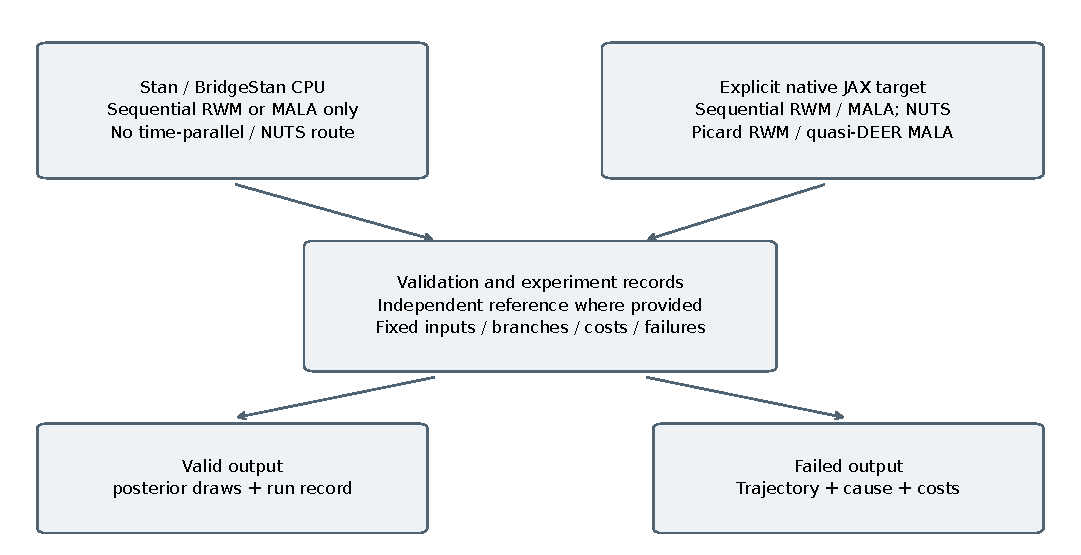
\includegraphics[width=\linewidth]{../../figures/software/architecture.pdf}
\caption{计算与验证流程。目标、核和执行器分别记录，失败轨迹与正常后验对象分离。NUTS 使用自身随机流及预热过程，不继承固定噪声 MH 的轨迹比较。该图是程序逻辑示意，不含性能预测。}
\end{figure}

\subsection{固定随机输入下的核}
MALA 的步长约定为
\begin{equation}
 y=q+h\nabla\ell(q)+\sqrt{2h}\,z,\qquad z\sim N(0,I_d).
\end{equation}
接受对数比包含正反向提议密度：
\begin{equation}
 a(q,y)=\ell(y)-\ell(q)-\frac{\|q-y-h\nabla\ell(y)\|^2-
 \|y-q-h\nabla\ell(q)\|^2}{4h}.
\end{equation}
当 $\log u<a(q,y)$ 时接受，否则保留 $q$。随机游走 Metropolis（RWM）使用 $y=q+s z$，接受对数比为 $\ell(y)-\ell(q)$。拒绝产生的自环计为一个转移。本文的 $h$ 不等于提议噪声标准差；这一约定在所有配对执行中固定。

随机输入由锁定 NumPy 版本下的 Philox 生成，采样与导数探测种子分开。比较固定的是噪声数组和对数均匀随机数组，而非跨软件的同名整数 seed。正式原始输出保存这些数组及其校验和。独立顺序 oracle 使用 NumPy 密度、解析梯度和显式循环，不调用待核验的 JAX 转移函数。

\subsection{两类时间执行}
quasi-DEER 执行器使用非重叠窗口。每轮以 Rademacher 向量和 Jacobian--向量积估计转移映射的对角导数，截断导数后通过仿射结合扫描更新窗口路径。接受事件在前向计算中仍是硬分支，导数采用 sigmoid 直通构造。与上游实现相比，本版改变了窗口调度和停止判据，且不使用 NaN 归零或状态裁剪；因此称为基于 quasi-DEER 的适配实现，不将其性能等同原论文。

设 $F_t$ 为固定实际随机输入下的硬转移映射，数值停止要求
\begin{equation}
 r=\max_{t,j}\frac{|q_{t,j}-F_t(q_{t-1})_j|}
 {\mathrm{atol}+\mathrm{rtol}|F_t(q_{t-1})_j|}\leq1.
\end{equation}
这里的残差控制局部递推一致性，既不是整条路径误差界，也不是统计无偏性证明。正式实验同时执行独立路径和接受事件核验，容差设为 $\mathrm{atol}=\mathrm{rtol}=10^{-10}$。独立审计另要求接受事件零失配，且每链无约束路径最大绝对差不超过 $100[\mathrm{atol}+\mathrm{rtol}\max(1,\max|q|)]$；100倍系数是预先固定的数值检查阈值，不是传播界。容差求解与独立核验成本均保留。

Online Picard 根据增量映射独立实现。固定 RWM 噪声后，接受增量只能为 $s z_t$ 或零；并行计算旧猜测下的增量，经前缀和产生候选路径，再在新前驱状态下复核接受事件。最长一致增量前缀用于推进滑动窗口。数学上的增量一致性与浮点逐位相等不同，本文只报告数值路径差和事件一致性。

\begin{figure}[htbp]\centering
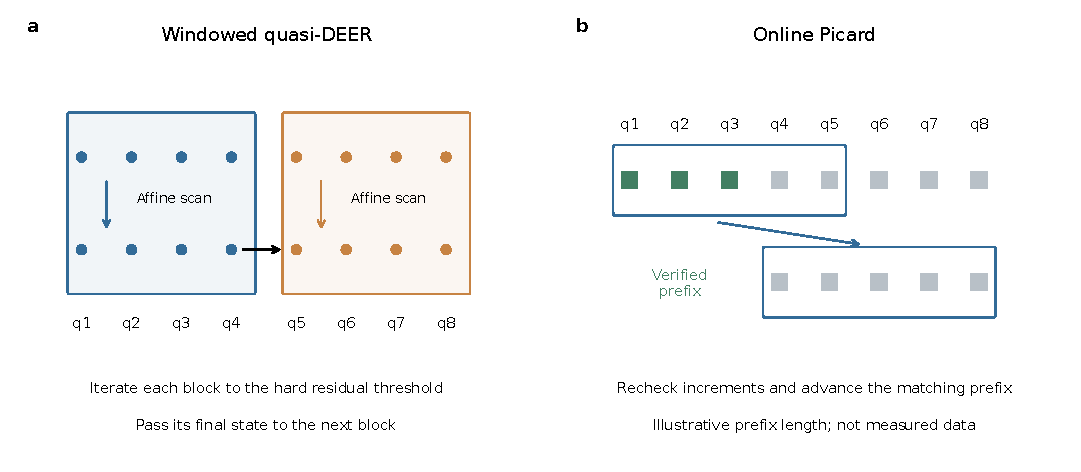
\includegraphics[width=\linewidth]{../../figures/software/methods.pdf}
\caption{两种执行器的调度示意。左侧按非重叠窗口迭代，每轮通过仿射扫描更新该窗口路径，停止后向下一窗口传递终点。右侧先并行计算增量，再根据新前驱复核接受事件，并推进最长一致前缀。绿色表示示意中确认的前缀。图中的窗口和前缀长度仅用于解释，不是实测轨迹，也不暗示固定迭代次数。}
\end{figure}

\subsection{失败与结果对象}
达到迭代上限、出现非有限状态或核验失配的轨迹不进入正常抽样对象。结果记录原始失败轨迹、残差、接受事件、求解次数、导数裁剪、确认长度和停止原因。MH 原型将非有限密度、梯度或提议视为失败；首版未一般地区分合法零密度提议与数值溢出。NUTS 保留 BlackJAX 的发散诊断，并在返回样本有限时保留其输出。两类数值事件分别报告，不能用统一的 ``completed'' 标签暗示收敛。

用户可以显式选择执行器停止失败后的顺序回退；独立审计失配或变换错误不触发该选项。回退复用原随机数组重新计算整个指定轨迹，保留并行阶段的失败及成本；不重抽随机数，也不选择较快完成的链。本文正式比较采用失败保留策略，不通过回退隐藏并行求解失败。约束输出仍须检查形状、有限性及可表示的支持集；审查中发现的边界处理修复以独立软件版本交付，冻结实验的源码归档保留。R 返回 $\texttt{iteration}\times\texttt{chain}\times\texttt{variable}$ 排列的 \texttt{posterior::draws\_array}，与独立运行记录配套。

\section{验证与开发证据}
软件测试覆盖密度、梯度、Jacobian、约束输出、固定噪声路径、接受事件、拒绝自环、部分窗口、迭代耗尽、非有限目标、内存守卫和共同随机输入回退。错误注入包括遗漏 Jacobian、改变尺度以及改变实际目标造成接受事件失配。协议与文件校验测试还检查重复任务跳过和输出损坏检测。有限测试不能替代一般正确性证明，但提供了可重放的反例检测机制。

冻结0.1.0通过43项Python测试和R包检查。审查修订版0.1.1进一步通过58项Python检查、R包检查及R到BridgeStan的端到端核验；后者的固定输入样本差为零。CPU主实验仍对应归档的0.1.0，新版边界修复不覆盖历史输出。高斯、logistic 与正值模型的 Stan/原生实现交叉核验通过；两个简单高斯目标上，上游固定提交的求解器与独立 MALA 参考的路径差小于 $10^{-8}$。这项复现仅检验上游求解器与指定映射的组合，不声称复现原文全部性能实验。

开发探测使用 G1、G2、L1、L2，固定转移数为 256 或 2048，窗口为 16、64、256，每组采用三个实际随机输入数组。192 项任务均完成，最大路径差为 $2.17\times10^{-9}$。Mac CPU 上的并行执行通常增加了时间；尤其是大数据 logistic 的多次梯度与导数求值成本明显。该探测属于开发资料，最早若干任务与初次 Stan 编译重叠，因此不用于正式速度推断。

小型生成式校准检查从 $\theta\sim N(0,1)$ 及八个 $y_i\sim N(\theta,1)$ 生成 12 个独立数据集，每个数据集运行五种工作流。后验具有解析均值 $\sum_i y_i/9$ 和标准差 $1/3$。60 次拟合均完成，MALA 的顺序/并行秩直方图相同，RWM 的顺序/并行结果也相同。该重复数下，观察到的区间覆盖不能确证校准；秩抽样的相关性和有限功效须继续检查。正式 SBC 使用另一组 64 个生成数据集和独立种子，避免把已观察的开发样本作为未见验证资料。

在正式SBC拟合开始前，另冻结依赖数据的对数似然统计量 $f_y(\theta)=-\tfrac12\sum_i(y_i-\theta)^2$，并从同一批保存样本计算其秩和解析后验期望误差。秩每32步取一个样本，共64个；与真参数处统计量相等的样本单独计数，以独立Philox流在并列范围内随机化秩。此伴随分析不改变拟合协议，也不据有限、仍可能相关的秩宣布一般校准通过。

\section{冻结实验设计}
\subsection{目标族与基线}
\begin{table}[htbp]\centering\small
\begin{tabular}{lll}\toprule
目标 & 定义 & 比较作用\\\midrule
G1 & 8 维标准高斯 & 简单几何与执行开销\\
G2 & 64 维旋转高斯，条件数 100 & 耦合与尺度差异\\
L1/L2 & 8 参数 logistic，样本量 256/4096 & 似然计算量\\
H1/H2 & 9 维漏斗，中心化/非中心化 & 相同分布的坐标与预热效应\\
A1 & 64 维潜在 AR(1) 高斯后验 & 高维相关结构\\
M1 & 8 维对称双峰高斯混合 & 跨模式探索压力\\\bottomrule
\end{tabular}
\caption{正式目标库。H1/H2 属于同一模型族；L1/L2 是同类回归的计算量变化。数据由记录的随机规则生成。本研究不把这些变体当作独立应用领域。}
\end{table}

五种工作流为顺序 MALA、窗口 quasi-DEER MALA、顺序 RWM、Online Picard RWM 和 BlackJAX NUTS。各工作流均采用四链；MH 使用预先固定步长，前 512 步作为丢弃段，随后保留 256 或 2048 步。NUTS 单独预热 512 步后保留相同数量，最大树深为 8。所有初始化固定为零，步长表、数据、随机种子及运行顺序写入机器可读协议。比较的对象是这些指定工作流，不能外推为经过全局最优调参的算法排名。

正式协议在独立探测后冻结，每组 24 次独立重复，共 1920 项任务。主实验不依据有利结果追加重复或选择模型。原研究计划提出的误差 MCSE 相对阈值 0.1 并未被承诺对每个压力目标满足；本版冻结有限重复数并完整报告其不确定性，区间跨阈值时保留为未判定。没有训练自动配置选择器，也没有将已见模型声明为选择器留出集。

\subsection{误差与参考}
对预先规定的函数集合 $\mathcal F$，以独立重复评价
\begin{equation}
 \widehat E_a(N)=\max_{f\in\mathcal F}\frac1R\sum_{r=1}^R
 \left(\widehat\mu_{a,f}^{(r)}(N)-\mu_f\right)^2/s_f^2.
\end{equation}
高斯目标使用标准化首坐标的均值、二阶矩及超过 1 的概率。漏斗目标使用标准化尺度变量、其双曲正切、局部变量的符号事件及条件标准化变量的余弦；这避免依赖漏斗局部变量的巨大高阶矩。双峰目标同时检查模式占比和连续函数。Logistic 检查前两个参数、截距的 logistic 变换及符号事件。全部函数与尺度在协议中明确，尺度统一取 1。

解析目标使用真实期望。L1/L2 的参考分别来自四次独立 NUTS 拟合，每次四链、预热 1024 步、保留 16384 步；参考种子与正式实验分离。两目标参考均未记录发散，L1的所检查函数及L2的连续函数 split-$\hat R$ 接近1，非退化函数参考MCSE最大约为 $7.6\times10^{-4}$。原协议计算所选函数的经典split-$\hat R$；审查后从相同保存样本补充秩正态化/折叠split-$\hat R$、bulk ESS和tail ESS，后文单列，不替换原分析。L2符号事件在全部参考样本中为零，其Rhat不可判定、参考误差未确定；不把零经验方差当作已证实的精度。参考 MCSE 取拟合间估计与批均值估计的较大值；该规则并不排除共同偏差。对这两个目标的结果称为参考平方差，不把它解释为无偏真实 MSE，也不无条件减去参考方差。

不确定性采用独立重复层面的 4000 次重采样，报告逐点 95\% 区间；每次重采样先在重复间求平方误差均值，再在预声明函数间取最大值。对可用共同参考另做正态、对角协方差扰动的敏感性传播，同一次扰动在所有重复中共用。它没有估计函数之间的完整参考协方差，不等于联合误差的精确传播；基本重复bootstrap区间另行保留。区间不是跨模型、方法和预算的同时置信保证。失败率、成功输出上的条件误差及全部成本分别呈现，有失败时不宣称无条件精度达标。

\subsection{计时与资源}
本地实验在 M4 Mac mini、16 GB 内存和 JAX CPU 后端上执行，使用 float64、JAX 0.6.2、BlackJAX 1.2.5、NumPy 2.2.6 和 BridgeStan 2.7.0。外层同一时刻运行一个实验任务。目标平台是整台指定机器，未将逻辑 CPU 个数直接解释为独占物理核预算。正式计算期间同机还进行了少量软件核验与文档生成，未实现全程独占空闲系统；保留全部原任务，不依据这种背景活动剔除计时值。

显式同步设备后结束执行计时。记录 JIT 编译、输入、NUTS 预热、执行、传输、独立核验和回退；逐任务墙钟还包含建模和写盘。本文以逐任务墙钟扣除额外计时重放成本、加上后验函数摘要与诊断计算时间，定义完整工作流时间；建模、原始数组写盘和校验和计算均在该口径内，另保留纯采样接口计时。完成初次执行后对同一编译程序进行两次缓存内重放，作为执行机制计时探测，额外成本单列；它们不是新的统计重复，也不计作增加后验样本。进程导入和一次性软件安装不是单次任务计时的一部分，因此本文不将该口径称为全新进程冷启动。

MH 的步长与窗口作为指定工作流的输入；开发探测属于离线研究费用，单独保留，不在每个正式拟合中重复摊入。NUTS 的逐次适配则包含在预热成本中。因此完整工作流比较回答的是给定配置的运行成本，尚未覆盖未知新模型上选择MH参数所需的成本，不应称为自动调参方案之间的完整费用比较。

CPU 内存为采样API期间每20 ms记录的进程绝对RSS峰值，包含先前驻留分配，未覆盖建模、写盘和子进程；本研究不评价GPU内存。数组空间有事前保守预算检查，数值迭代上限保留。运行没有人为总时长截止。冻结源代码和协议校验和、随机化任务顺序、逐任务原始数组与状态支持中断后恢复；成功与失败结果均保留。

\section{正式结果与范围}
本机按冻结协议登记了 1920 项正式任务，全部结束，其中 0 项未返回满足输出标准的正常样本。失败计数与原始输出均保留；该总任务数包含配对执行，并非 1920 个独立模型。每个模型、预算及工作流的独立重复数为 24。

正常输出中，独立核验记录的最大数值路径差为 $2.36\times10^{-8}$，接受事件失配总数为 0。这一陈述以数值核验及当前目标库为边界，不构成一般轨迹或平稳分布证明。

quasi-DEER MALA 的模型—预算组中位缓存执行速度比范围为 0.0192 至 0.174，研究审计工作流速度比范围为 0.0715 至 0.739。速度比定义为同核顺序时间除以并行时间，小于 1 表示并行执行更慢；这里只统计成对有效输出，失败另行报告。

Online Picard RWM 的模型—预算组中位缓存执行速度比范围为 0.0503 至 0.809，研究审计工作流速度比范围为 0.226 至 0.814。速度比定义为同核顺序时间除以并行时间，小于 1 表示并行执行更慢；这里只统计成对有效输出，失败另行报告。

\begin{figure}[htbp]\centering
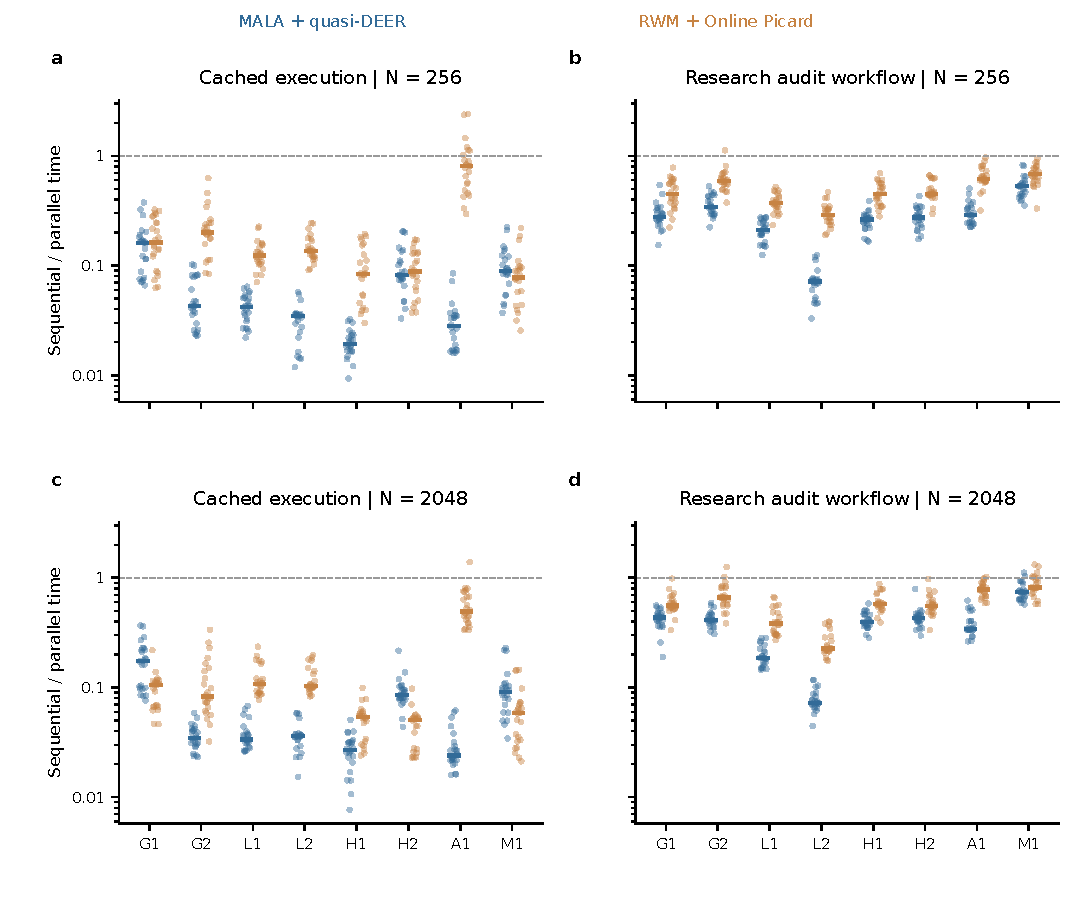
\includegraphics[width=\linewidth]{../../figures/software/paired-costs.pdf}
\caption{同核成对成本。上、下行分别为每链保留256和2048步；左列为两次缓存重放时间的中位数之比，右列为含编译、预热/丢弃段和独立核验的工作流时间比。每个点为一个独立重复中的配对比，短线为组中位数；同一轨迹的计时重放不当作统计重复。虚线表示速度比1。任何缺失配对均在原始任务及失败表中保留。}
\end{figure}

表中列出较大预算下的函数最大平方误差。L1/L2 采用有限参考，因此相应数值是参考平方差。完整逐函数误差、逐点区间、参考敏感性区间、失败比例区间及两预算结果随机器可读材料交付。不能把表中的最小数值自动解释为确定排名。

\begin{table}[htbp]\centering\small\setlength{\tabcolsep}{3pt}\begin{tabular}{lrrrrr}\toprule

目标 & 顺序MALA & quasi-DEER & 顺序RWM & Picard & NUTS\\\midrule

G1 & $0.00199$ (0) & $0.00199$ (0) & $0.00542$ (0) & $0.00542$ (0) & $0.000531$ (0)\\

G2 & $0.125$ (0) & $0.125$ (0) & $0.164$ (0) & $0.164$ (0) & $0.000322$ (0)\\

L1 & $0.000255$ (0) & $0.000255$ (0) & $0.000673$ (0) & $0.000673$ (0) & $1.46\times10^{-5}$ (0)\\

L2 & $6.22\times10^{-6}$ $\dagger$ (0) & $6.22\times10^{-6}$ $\dagger$ (0) & $1.91\times10^{-5}$ $\dagger$ (0) & $1.91\times10^{-5}$ $\dagger$ (0) & $2.28\times10^{-7}$ $\dagger$ (0)\\

H1 & $0.138$ (0) & $0.138$ (0) & $0.131$ (0) & $0.131$ (0) & $0.112$ (0)\\

H2 & $0.0215$ (0) & $0.0215$ (0) & $0.0376$ (0) & $0.0376$ (0) & $6.11\times10^{-5}$ (0)\\

A1 & $0.00803$ (0) & $0.00803$ (0) & $0.856$ (0) & $0.856$ (0) & $0.000665$ (0)\\

M1 & $0.252$ (0) & $0.252$ (0) & $0.359$ (0) & $0.359$ (0) & $0.296$ (0)\\

\bottomrule\end{tabular}\caption{每链保留2048步时的最大函数平方误差/参考平方差。括号内为该组24次重复中的输出失败数；有失败时，误差仅描述成功输出。误差不包含失败的假定损失，不代表无条件达标。$\dagger$表示参考精度未确定，该行仅展示参考平方差，不能判断全函数精度达标。}\end{table}

按前述工作流口径汇总，正式尝试合计耗时 5080.9 秒，其中失败任务耗时 0.0 秒。另有缓存计时重放开销5711.5秒，完整保留但不重复计入单次工作流成本。逐组成本及全部失败分母另存分析结果。

NUTS 在 46 个已返回有限样本的任务中记录到发散，总计 2358 个保留转移的发散事件。发散与数值输出失败分别呈现，不能因为数组有限而删除这一诊断。多峰和漏斗目标上的误差须结合模式占比及尺度函数理解。

NUTS另有6861个保留转移达到255个积分步的设定上限；积分步数及逐次适配参数随原始记录保存。

采样接口期间记录的逐任务进程RSS峰值范围为244.3至549.0 MiB；它包含进程已驻留内存，只覆盖接口调用阶段，不能解释为每种算法的独占增量内存或整项任务的严格峰值。

quasi-DEER的模型—预算组中，单个输出转移对应的前向转移映射求值次数中位数范围为14.58至66.15，顺序MH为1。

Online Picard的模型—预算组中，单个输出转移对应的前向转移映射求值次数中位数范围为2.00至21.38，顺序MH为1。

这些程序层面的映射调用计数包含丢弃段和拒绝自环，尚不包含独立审计；它们不是浮点运算量或密度/梯度调用次数。quasi-DEER的JVP另存，因此不能仅据调用数精确分解运行瓶颈。

\begin{figure}[htbp]\centering
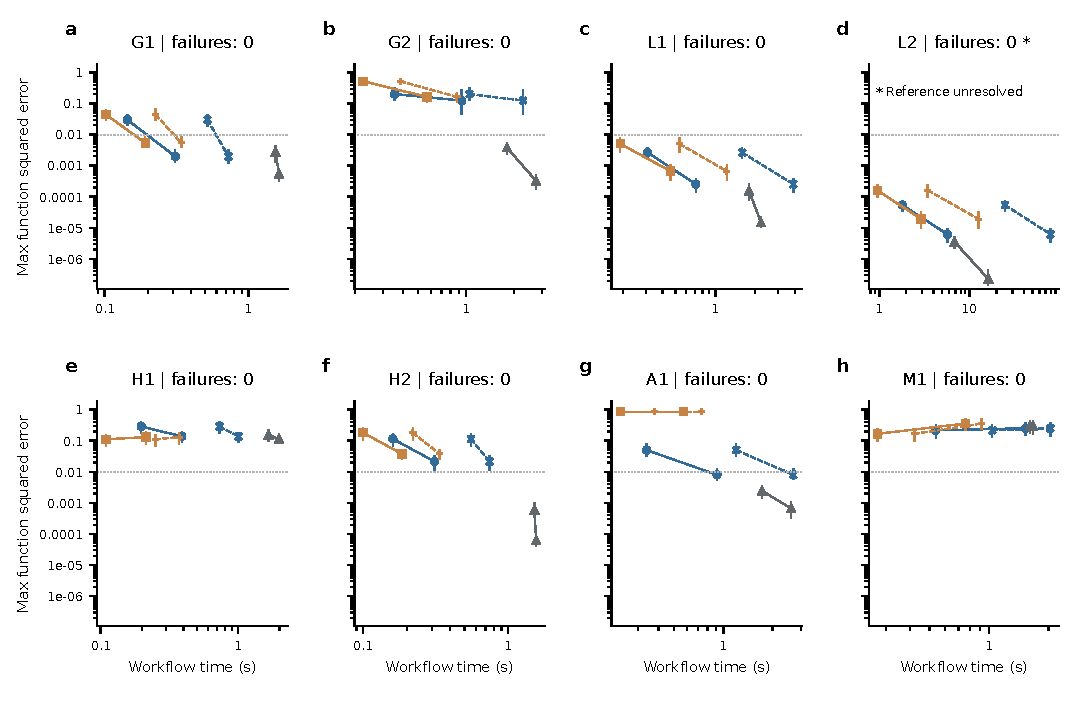
\includegraphics[width=\linewidth]{../../figures/software/error-cost.pdf}
\caption{固定采样计划的误差—成本关系。横轴为成功输出条件下的工作流时间中位数，全部尝试和失败成本另表保存。每条线连接同一指定工作流的两个预算点，不表示中间预算已被测量。蓝色为MALA、橙色为RWM、灰色为NUTS；实线/圆或方形为顺序MH，虚线/叉号为相应时间执行器，三角形为NUTS。误差取预声明函数中最大的重复平均平方误差；L1/L2为有限参考平方差。线段区间为逐点95\%重复重采样区间，有限参考的共同误差敏感性另行传播；传播采用正态对角协方差工作假设，非同时保证。星号表示参考精度未确定，该面板仅供探索性平方差比较。面板标题列出该模型全部正式任务中的输出失败数，失败组的误差为条件结果。点虚线标出0.01作为预声明误差阈值。}
\end{figure}

\noindent mala/sequential在较长预算、$\epsilon=0.1$下的逐点判断为：区间低于阈值2个目标，区间高于阈值4个，跨阈值1个，参考或输出条件不足1个。\par

\noindent mala/quasi\_deer在较长预算、$\epsilon=0.1$下的逐点判断为：区间低于阈值2个目标，区间高于阈值4个，跨阈值1个，参考或输出条件不足1个。\par

\noindent rwm/sequential在较长预算、$\epsilon=0.1$下的逐点判断为：区间低于阈值2个目标，区间高于阈值5个，跨阈值0个，参考或输出条件不足1个。\par

\noindent rwm/online\_picard在较长预算、$\epsilon=0.1$下的逐点判断为：区间低于阈值2个目标，区间高于阈值5个，跨阈值0个，参考或输出条件不足1个。\par

\noindent nuts/sequential在较长预算、$\epsilon=0.1$下的逐点判断为：区间低于阈值5个目标，区间高于阈值2个，跨阈值0个，参考或输出条件不足1个。\par

这些判断仅对应两个已测量预算中的较长预算，不构成同时置信结论，也不提供单次运行可观测的停止规则或精确的达标时间。

正式生成式检查完成64个新数据集、五种工作流，共320次拟合，其中0次输出失败。90\%后验区间的覆盖估计及其二项区间按数据集作为独立单位报告；保留所有秩与原始样本。抽稀秩仍可能相关，这一检查不提供一般SBC一致性证明。

\noindent mala/sequential：覆盖率 0.844，95\%二项区间 [0.731, 0.922]。\par

\noindent mala/quasi\_deer：覆盖率 0.844，95\%二项区间 [0.731, 0.922]。\par

\noindent rwm/sequential：覆盖率 0.828，95\%二项区间 [0.713, 0.911]。\par

\noindent rwm/online\_picard：覆盖率 0.828，95\%二项区间 [0.713, 0.911]。\par

\noindent nuts/sequential：覆盖率 0.828，95\%二项区间 [0.713, 0.911]。\par

正式生成式检查另记录到0个保留转移的发散事件，涉及0次拟合；该诊断与输出失败分开保存。

本次覆盖率点估计均低于名义90\%，而相应二项区间均包含90\%。这一有限重复结果既不能证明完全校准，也不应被改写为已确证系统性覆盖不足。

对数似然测试量也完成320次拟合的伴随分析，共记录0个秩并列。逐方法秩直方图、抽稀后相关性及解析期望误差随原始数据交付；这些描述性诊断不构成统一性检验或正确性证书。

L2 的参考符号事件在262144个相关样本中均为零，Rhat 对该函数不可判定，不能把零经验方差当作事件概率已被精确确定。因此保留原函数集合，并将L2全函数精度判定标记为未确定。没有通过删除该函数得到达标结论。

上述结果来自历史Mac CPU协议，不包含后续Windows实验；原生Windows实现及其独立协议的实测结果在后文另行报告。


\section{审查后的伴随分析与CPU机制实验}
\subsection{版本与扩展验证}
CPU主实验保留0.1.0源代码和原协议；0.1.1增加约束输出检查、末窗口有效步掩码、错误及失败记录，并修复R单元素数组。变换检查和掩码可能影响计时，不能用旧性能代表新版。审查后对8目标、5工作流各取原较短预算的第一个重复，旧/新源码分别执行；MH复用保存的实际随机数组，NUTS复用锁定随机流。40组均返回有效输出，最大路径差为$1.99\times10^{-13}$，接受事件零失配。这是有限数值对照，不是性能等价或边界正确性证明。

新增Poisson回归示例无需改动内核，公开模型对象分别实现JAX密度与独立NumPy密度/解析梯度，先验证坐标和导数，再比较固定输入的四种MH工作流。密度与梯度最大差约$2.84\times10^{-14}$；MALA和RWM配对最大路径差分别为$7.90\times10^{-11}$和$3.61\times10^{-16}$，接受事件无失配。示例旨在说明扩展和核验，不作为新性能或后验收敛证据。

\subsection{同数据集的解析SBC对照}
本节为审查后伴随分析，未追溯为原协议预声明检验。64组真参数和数据已保存，后验为$N(\sum_j y_j/9,1/9)$，故直接计算解析90\%区间，无需新增拟合。解析区间覆盖54/64，点估计0.84375，95\%二项区间为[0.731,0.922]。五种工作流共享同64组数据，同核顺序/并行还共享轨迹，因此不能当作五次独立校准证据。

\begin{table}[htbp]\centering\small\setlength{\tabcolsep}{4pt}
\begin{tabular}{lrrrrrr}\toprule
工作流 & 覆盖数 & 分歧数 & 下端点RMSE & 上端点RMSE & 均值RMSE & 标准差RMSE\\\midrule

顺序MALA & 54 & 4 & 0.0179 & 0.0195 & 0.0105 & 0.0063\\

quasi-DEER & 54 & 4 & 0.0179 & 0.0195 & 0.0105 & 0.0063\\

顺序RWM & 53 & 3 & 0.0318 & 0.0267 & 0.0147 & 0.0107\\

Picard & 53 & 3 & 0.0318 & 0.0267 & 0.0147 & 0.0107\\

NUTS & 53 & 3 & 0.0222 & 0.0190 & 0.0115 & 0.0078\\

\bottomrule\end{tabular}
\caption{同64数据集的配对解析对照。RMSE按数据集计算；分歧指解析与MCMC区间对同一真参数的覆盖判断不同，不能只据总体覆盖率相等判定区间相等。}
\end{table}
MALA的分歧数据集编号为23、32、36、56，RWM为26、32、56，NUTS为11、26、36（从0编号）。例如MALA有2例解析覆盖而MCMC未覆盖、另2例相反，抵消后总覆盖数相同。该批解析覆盖本身偏低，与有限生成样本波动的解释相容；端点及后验矩误差仍显示有限链估计差异，不能据此证明无额外采样偏差。

\subsection{现代诊断与有限预算误差的对应}
从全部1920项保存样本及8次参考拟合提取每个参数和预声明函数，以posterior 1.7.0计算秩正态化/折叠split-$\hat R$、bulk ESS与tail ESS\cite{posterior}。每个拟合分别计算，结果不替换原经典函数诊断；常量链等不可判定值保留为空。表中汇总NUTS，全80组的逐拟合、逐变量诊断随复现材料交付。

\begin{table}[htbp]\centering\scriptsize
\begin{tabular}{lrrrrrrl}\toprule
目标/$N$ & 发散\% & 上限\% & 最大$\hat R$ & 最小bulk ESS & 最小tail ESS & 函数误差 & 判据\\\midrule

A1/256 & 0.00 & 0.00 & 1.018 & 496.4 & 469.7 & 0.00243 & 低于阈值\\

A1/2048 & 0.00 & 0.00 & 1.002 & 5576.0 & 5186.4 & 0.000665 & 低于阈值\\

G1/256 & 0.00 & 0.00 & 1.018 & 1198.4 & 461.8 & 0.00271 & 低于阈值\\

G1/2048 & 0.00 & 0.00 & 1.003 & 11148.1 & 5316.6 & 0.000531 & 低于阈值\\

G2/256 & 0.00 & 0.00 & 1.015 & 636.5 & 448.0 & 0.00383 & 低于阈值\\

G2/2048 & 0.00 & 0.00 & 1.002 & 5848.5 & 5429.4 & 0.000322 & 低于阈值\\

H1/256 & 0.71 & 2.67 & 1.745 & 6.3 & 8.0 & 0.154 & 高于阈值\\

H1/2048 & 1.11 & 3.16 & 1.273 & 11.4 & 5.4 & 0.112 & 高于阈值\\

H2/256 & 0.00 & 0.00 & 1.018 & 815.5 & 545.5 & 0.000595 & 低于阈值\\

H2/2048 & 0.00 & 0.00 & 1.002 & 7125.8 & 5438.9 & 6.11e-05 & 低于阈值\\

L1/256 & 0.00 & 0.00 & 1.017 & 358.2 & 393.2 & 0.000154 & 低于阈值\\

L1/2048 & 0.00 & 0.00 & 1.003 & 3459.7 & 4381.6 & 1.46e-05 & 低于阈值\\

L2/256 & 0.00 & 0.00 & 1.019 & 507.4 & 532.0 & 3.52e-06 & 不可判定\\

L2/2048 & 0.00 & 0.00 & 1.002 & 4243.8 & 5109.4 & 2.28e-07 & 不可判定\\

M1/256 & 0.00 & 0.00 & 1.738 & 6.2 & 30.6 & 0.301 & 高于阈值\\

M1/2048 & 0.00 & 0.00 & 1.734 & 6.1 & 26.8 & 0.296 & 高于阈值\\

\bottomrule\end{tabular}
\caption{NUTS按模型和保留预算分组的伴随诊断。发散和上限命中以24次拟合、各4链的全部保留转移为分母；$\hat R$为参数与拟合中的最大值，ESS为最小值。函数误差为原预声明最大平方误差/参考平方差，判据对应原逐点95\%区间与0.01阈值，不由诊断阈值重定义。}
\end{table}
2358次发散与6861次积分上限命中均来自中心化漏斗H1：短/长预算分别为174/2184次发散及657/6204次上限命中。双峰M1无发散，却在两个预算下都有约1.73的最大参数$\hat R$，所选函数误差亦高于阈值。五个目标的长预算函数误差区间低于阈值，与H1/M1的探索问题分别成立；L2参数诊断良好不消除参考符号事件恒零的不确定性。特定函数误差小、无发散和后验全面探索是不同陈述。

\subsection{三种成本口径}
缓存执行衡量已编译内核；正常推断应包含必要建模、编译、预热、转换及诊断；研究审计另加入独立顺序参考和完整数组、校验和归档。历史时钟未单独测量正常输出与所有建模步骤，故只能以$T_{\rm API}-T_{\rm independent}+T_{\rm diagnostic}$给出内存内正常使用的记账估计，不能冒称重新实测的完整正常工作流。该估计不含未分离的建模、R转换和持久化费用。

\begin{table}[htbp]\centering\small\setlength{\tabcolsep}{4pt}
\begin{tabular}{lrrr}\toprule
执行器 & 缓存执行 & 正常内存口径估计 & 研究审计工作流\\\midrule

quasi-DEER & 0.019--0.174 & 0.038--0.175 & 0.072--0.739\\

Picard & 0.050--0.809 & 0.110--0.393 & 0.226--0.814\\

\bottomrule\end{tabular}
\caption{历史主实验中，各模型--预算组的配对速度比中位数范围。三列均为顺序时间/并行时间；中列是不同包含项的记账敏感性分析，不与另外两列混称三种完整实测工作流。}
\end{table}
共享审计成本使速度比向1靠近，可能掩盖加速或减速；当前缓存与去独立核验的估计口径也均未显示组中位加速，因此负结果不能仅归因于审计。新增机制实验另直接计量\texttt{audit=False}的建模、采样与基本均值/方差/链间诊断，并单列普通样本输出耗时；它是最小Python正常工作流，不包含R转换及现代posterior诊断，也不是全新进程冷启动。

\subsection{小型CPU机制实验}
审查后另冻结\texttt{cpu-mechanism-v1}，使用0.1.1，目标G1/G2/L1、链数1/4、窗口16/64、每链256步、两组成对MH执行方式和每格3个新实际随机数组，共72项任务。沿用主协议的指定核参数，冻结随机顺序；没有按速度追加或删除任务。每次至少7次缓存计时重放、总观测窗口至少0.2秒，作为技术重复而非独立统计重复。全部72项完成；分段重放与生产程序首链的接受事件无失配。

生产执行另外记录进程CPU秒/墙钟秒和10毫秒间隔系统利用率。组中位进程占用约为1.00--2.99个CPU核当量，测量包含运行返回和监测开销，不是物理核心绑定，也不能将\texttt{vmap}当作指定核心数的证明。固定前驱状态的微基准比较串行映射与向量化映射在同一批状态、噪声上的吞吐；它没有MCMC的递推依赖，不能将吞吐比直接当作轨迹加速比。

\begin{figure}[htbp]\centering
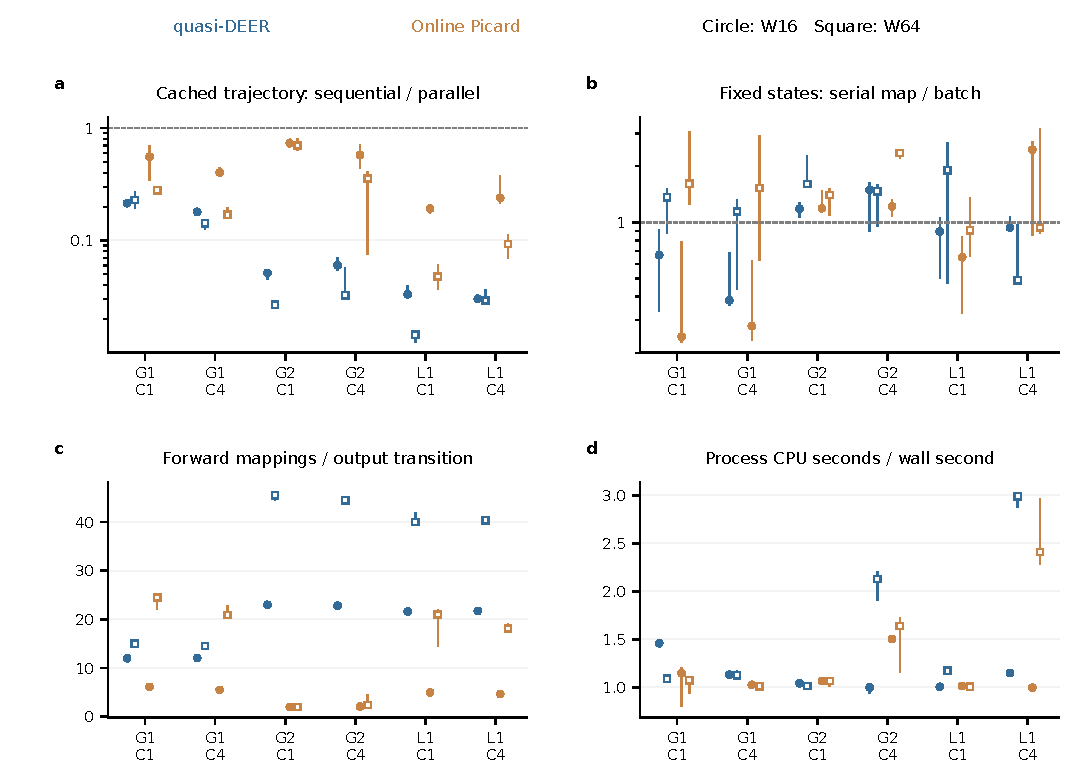
\includegraphics[width=\linewidth]{../../figures/software/cpu-mechanism.pdf}
\caption{新冻结的72项机制任务。每格3个实际随机数组，符号为组中位数，细线为最小至最大值；技术计时重复不扩大样本量。蓝色为quasi-DEER，橙色为Picard；圆点为窗口16，方形为64；横轴C为链数。a：缓存轨迹速度比，1以上才为加速。b：固定状态批量吞吐比，1以上表示批处理有利，但它不是轨迹加速。c：每个输出转移的前向映射求值数，quasi-DEER还另有JVP；拒绝自环计入转移。d：进程CPU秒/墙钟秒，表示观测消费量而非核数配置。}
\end{figure}

quasi-DEER的组中位缓存速度比为0.0145--0.23，固定状态批量吞吐比为0.381--1.91；每转移前向映射数为12--45.5，另有5.5--22.2次JVP。

Picard的组中位缓存速度比为0.0477--0.732，固定状态批量吞吐比为0.244--2.46；每转移前向映射数为2--24.5。

这些量显示局部批量求值收益与完整轨迹重复工作之间的差距，而非证明单一瓶颈。例如G1、四链Picard把窗口从16增至64时，首链每轮确认数的组中位数均约5.57，前向工作却从5.50增至20.88次/转移，缓存速度比由0.402降至0.170。G2、单链quasi-DEER的平均每窗口轮数由11增至22.25，前向工作从23增至45.5次/转移，速度比由0.051降至0.027。窗口扩大会增加可批处理宽度，但确认推进和求解轮数决定有效工作效率；这些例子是冻结小网格中的观察，尚未识别正加速的交叉点。

为审查阶段组成，另将首链实现拆成单独编译的批量求值/JVP、扫描和接受复核，并记录每轮残差或确认前缀。拆分插入同步及Python控制，改变了融合执行。所得控制及未细分部分比例很高，不能据此宣称生产程序主要受Python控制限制；它暴露了分段探针的扰动。全部阶段秒数和原始逐轮记录公开，可用于复查数值过程；对生产程序的精确XLA剖面仍属于局限。三次独立重复及短微基准不足以给出普遍硬件因果结论。

\subsection{可移植复现检查}
另建锁定依赖的Python环境并安装非editable轮子，在迁移目录运行完整测试。首次57项通过、1项因漏带上游比较源文件而失败；补齐许可与该源文件后，仅复查失败项并通过，保留初次失败日志。迁移目录的新目标示例也通过。R包检查日志与显式\texttt{PB\_RUN\_INTEGRATION=1}的3项集成测试日志分别交付，后者实际执行15个断言，不以默认跳过替代通过。

迁移目录从1920项主实验、8次参考拟合和320项SBC原始证据重建主摘要，逐字节一致。三个归档含全部源代码、协议、原始数组和论文输入；新临时目录解压后，校验、分析、1928项现代诊断重算、绘图和编译均通过，诊断值排除耗时后逐项一致。检查仍共享Mac、R库和编译器，不等同外部团队或异构系统复现。



\section{解释、限制与复现}
目前证据支持的是一个能够区分目标一致性、轨迹求解与统计精度的研究实现。CPU正式比较中，两种时间执行器均未取得组中位工作流加速；前向映射调用增加与这一结果一致，说明额外求值和导数计算可能抵消可利用的并行位置。新增机制测量进一步将批处理吞吐、重复求值与分段调度区分；由于分段执行插入同步，不能把其阶段比例直接当作生产程序的精确剖面。编译策略和底层运算仍限制因果归因。Picard原文在Apple M3 CPU上对昂贵延迟微分方程似然报告约2.52倍墙钟加速\cite{grazzi}；这与本研究的低成本合成目标不同。上游算法的窗口策略、停止规则和计时排除项亦不同，因此当前负例不能解释为CPU普遍不适合时间并行，也不识别正加速的分界。

合成模型使目标、真值和失败机制更易核对，同时限制了应用外推。中心化与非中心化漏斗可对照几何，但不能代替真实层次数据分析；潜在 AR(1) 仍具有高斯后验；双峰任务的有限样本模式比例也不证明普遍探索能力。正式结果应据函数、预算和诊断逐项阅读，不能由短链 ESS 或执行器返回成功推断可靠推断已经完成。

quasi-DEER 的局部残差加独立轨迹核验是一种计算上可审查的约束，仍没有提供从容差到一般后验函数偏差的理论界。接受分支接近阈值时，浮点差异可能改变事件；因此本文保存事件差与失败而不以统一 API 隐去保证类别。Online Picard 同样受浮点前缀和与窗口调度影响。本版顺序回退重新计算全路径，尚未优化为仅重算未确认后缀。

本研究仅评价指定CPU环境。原生Windows GPU后端尚未实现，不属于本版软件能力及实验结论；历史WSL2交接资料仅归档保留。自动配置模块未进入本版贡献，当前没有足够证据支持稳定收益区间。昂贵似然、真实数据应用和分散初始化属于后续研究；本轮不以挑选有利案例扩展结论。

\section*{代码、数据与辅助工具}
数据均由公开的项目生成规则产生，原始运行输出与协议存于本地研究项目，尚未上传公共仓库。软件安装源、实验/分析源、原始证据及论文构建材料分成三个互有关联的本地归档，提供根目录入口与逐文件校验和。独立依赖环境和迁移目录验证已在同一Mac完成，不等同另一研究团队或操作系统的复现。R包检查与显式开启集成测试的日志分开保存。R 包发布候选及 Python 内核随项目交付；上游 BSD 许可源码保留来源，Online Picard 按论文独立实现。本文使用生成式工具辅助代码、实验组织、图表与中文草稿，并用实际运行、独立实现和可重建原始输出核验相关陈述。稿件尚需研究者最终审阅、确认署名与投稿范围，不将工具列为作者。

\begin{thebibliography}{99}\small\setlength{\itemsep}{2pt}
\bibitem{zoltowski} Zoltowski D.M., Wu S., Gonzalez X., et al. \href{https://proceedings.nips.cc/paper_files/paper/2025/hash/202886ee1c9ca735cb5bff3a00a69883-Abstract-Conference.html}{Parallelizing MCMC Across the Sequence Length}. Advances in Neural Information Processing Systems, 2025, 38.
\bibitem{grazzi} Grazzi S., Zanella G. \href{https://doi.org/10.1093/biomet/asag022}{Parallel computations for Metropolis Markov chains with Picard maps}. Biometrika, 2026, 113(2): asag022.
\bibitem{stan} Carpenter B., Gelman A., Hoffman M.D., et al. \href{https://doi.org/10.18637/jss.v076.i01}{Stan: A Probabilistic Programming Language}. Journal of Statistical Software, 2017, 76(1): 1--32.
\bibitem{bridgestan} BridgeStan contributors. \href{https://roualdes.us/bridgestan/latest/languages/python.html}{BridgeStan: Python interface documentation}. 本研究使用版本 2.7.0，构建来源与许可随代码归档。
\bibitem{blackjax} Cabezas A., Corenflos A., Lao J., Louf R., et al. \href{https://arxiv.org/abs/2402.10797}{BlackJAX: Composable Bayesian inference in JAX}. arXiv:2402.10797, 2024.
\bibitem{comparemcmcs} NIMBLE development team. \href{https://github.com/nimble-dev/compareMCMCs}{compareMCMCs: Tools for comparing MCMC efficiency from NIMBLE and other engines}. 软件作者仓库，访问于2026年10月3日；此处引用功能说明，未复现其性能。
\bibitem{pplbench} PPL Bench contributors. \href{https://github.com/facebookresearch/pplbench}{PPL Bench: Evaluation Framework for Probabilistic Programming Languages}. 软件作者仓库，访问于2026年10月3日。
\bibitem{posteriordb} Magnusson M., Torgander J., Bürkner P.-C., Zhang L., Carpenter B., Vehtari A. \href{https://proceedings.mlr.press/v258/magnusson25a.html}{posteriordb: Testing, Benchmarking and Developing Bayesian Inference Algorithms}. Proceedings of Machine Learning Research, 2025, 258:1198--1206.
\bibitem{posterior} Stan development team. \href{https://mc-stan.org/posterior/reference/rhat.html}{posterior: Rhat, bulk ESS and tail ESS documentation}. 本研究使用posterior 1.7.0；常量链诊断保留为不可判定。
\end{thebibliography}
\end{document}
